\documentclass[Main]{subfiles}
\begin{document}

\chapter{Hardware}

\section{System oversigt}

Til styring af drone, skal der laves en sender og modtager.

\begin{figure}[H]
\centering
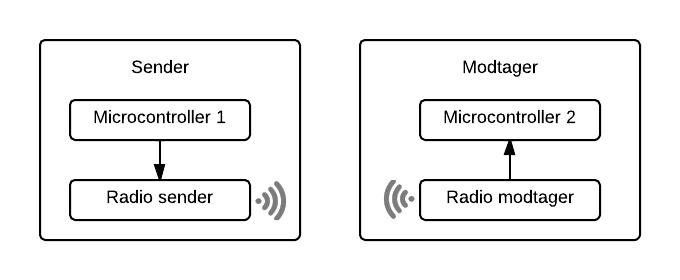
\includegraphics[scale=0.6]{Blokdiagram}
\caption{Skitse af hardware}
\end{figure}

\code{Sender} er den brugeren laver sit input på. 
\\ \code{Modtager} er den enhed der er sat på dronen, som skal modtage signalet fra senderen.\\
Det vil sige der skulle laves to enheder. Radioen er baseret på chippen cc1101 fra texas instruments. Microcontrolleren er en atmega8 fra Atmel Corporation.
\code{Senderen} skal også have knapper så brugeren kan lave sit input.

\section{Grænseflader}
De interne og eksterne grænseflader. 

Spi er designet i forhold til Atmels standarter. \cite{SPI}

\itoc/TWI er designet i forhold til Atmels standarter \cite{Twi}


\subsection{Sender}
\begin{figure}[H]
\centering
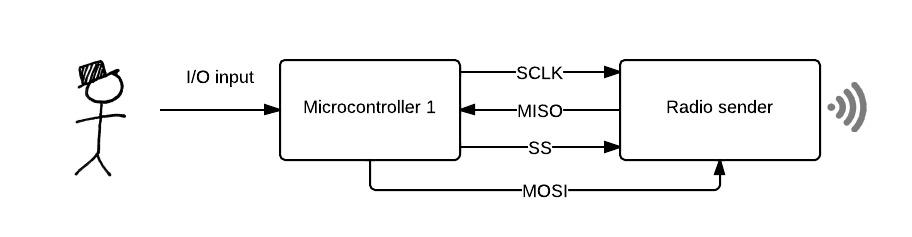
\includegraphics[scale=0.5]{SenderInterface}
\caption{Grænseflader for sender}
\label{fig: SenderInterface}
\end{figure}
På Figur \ref{fig: SenderInterface} ses et blokdiagram af senderen med alle grænseflader.
De eksterne grænseflader, er der hvor brugeren skal lave sit input. Det vil sige der er her han laver et programvalg som bliver sendt videre til dronen.
De interne grænseflader
Kommunikationen mellem microcontroller 1 og radiosenderen, forgår via SPI protokollen. 

Radio interfacet er beskrevet i sektionen Radio.



\subsection{Modtager}

\begin{figure}[H]
\centering
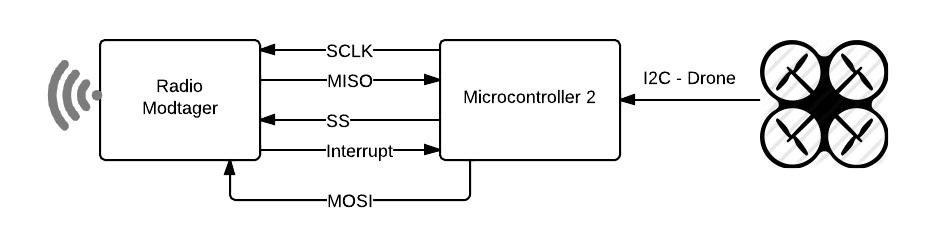
\includegraphics[scale=0.5]{ModtagerInterface}
\caption{Grænseflader for modtager}
\label{fig: ModtagerInterface}
\end{figure}
På Figur \ref{fig: ModtagerInterface} ses et blokdiagram af modtageren med alle grænseflader.
Radioen modtager en pakke fra senderen. Når hele pakken er modtaget laves et interrupt på microcontroller 2.

Microcontroller 2, henter hele pakken fra radioen og sætter den i modtage mode igen. 

Microcontroller 2, tager så de modtaget data fra radioen og putter dem i en output buffer til \itoc.

Radio interfacet er beskrevet i næste sekstion.


\subsection{Radio}
Opsætningen på radioen vi køre med er som følger:
\begin{itemize}
\item 433MHz radio frekvens
\item 2.5 kbps overførselshastighed
\item CRC af dataoverførslen
\item Benytter kanal 0 i 433MHz frekvensbåndet.
\end{itemize}


Framen der bliver sendt frem og tilbage ser ud som følger:
\begin{figure}[H]
\centering
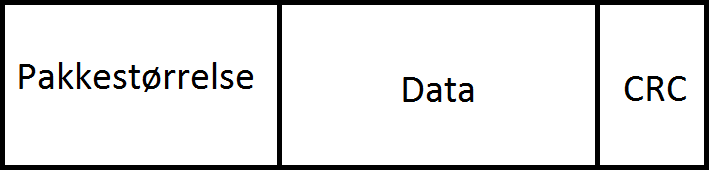
\includegraphics[scale=0.8]{Pakke}
\caption{Framens opbygningen}
\label{fig: Pakke}
\end{figure}

Pakkens opbygning;
Pakkestørrelse: Længden af den samlet pakke, eksklusiv crc delen. Grunden til denne skal med er at der bliver brugt variable pakke størrelse. Den kan også sættes til fixed længde og så er der ikke brug for denne.

Data: Dette er payloaden, det er her alle de informationer der skal sendes frem og tilbage ligger. Det vil sige at et program er valgt efterfulgt af hvilket program det er.

CRC: Er en checksum som sendes med. Den sikre at framen der kommer over ikke er corrupt.



\section{Design}
Det der skulle designes var
et print til sender og et til modtager.

\subsection{Sender}
Senderprintet indeholder knapper, en mega8 mikroprocessorer og en socket til radiosenderen.

Knappe designet er aktive lav, som det kan ses på Figur \ref{fig: Knapper}.


\begin{figure}[H]
\centering
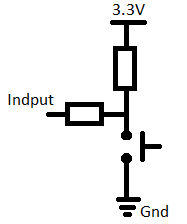
\includegraphics[scale=0.8]{Knapper}
\caption{Design af knapper}
\label{fig: Knapper}
\end{figure}

Disse knapper (Tach Switchs) er der 9 af i alt til styring af dronen.
Skematic af systemet kan ses i \cite{SenderSCM}.
\subsection{Modtager}
Modtagerprintet indeholder en mega8 mikroprocessorer og en radiosender.

Dette design indeholder en socket til radioen og en socket til \itoc forbindelsen til dronen.
Skematic af systemet kan ses i \cite{ModtagerSCM}.


\subsection{Strøm input}

Hele enheden køre på 3.3 V.
Der er ikke lavet noget beskyttelse på inputstrømmen så det skal være 3.3V dc.

Det totale strømforbrug for hele sender systemet er:
\begin{itemize}
\item 8mA pasiv, dvs når der ikke sendes
\item 43mA aktiv, dvs når der trykkes på en knap så data sendes til modtager.
\end{itemize}

Så det vil sige at senderen på et AA 2000mA batteri kan være på standby i $2000mA/8mA = 250 Timer$ eller sende i $2000mA/43mA = 46,5 Timer$


\section{PCB layout}

\begin{figure}[H]
\centering
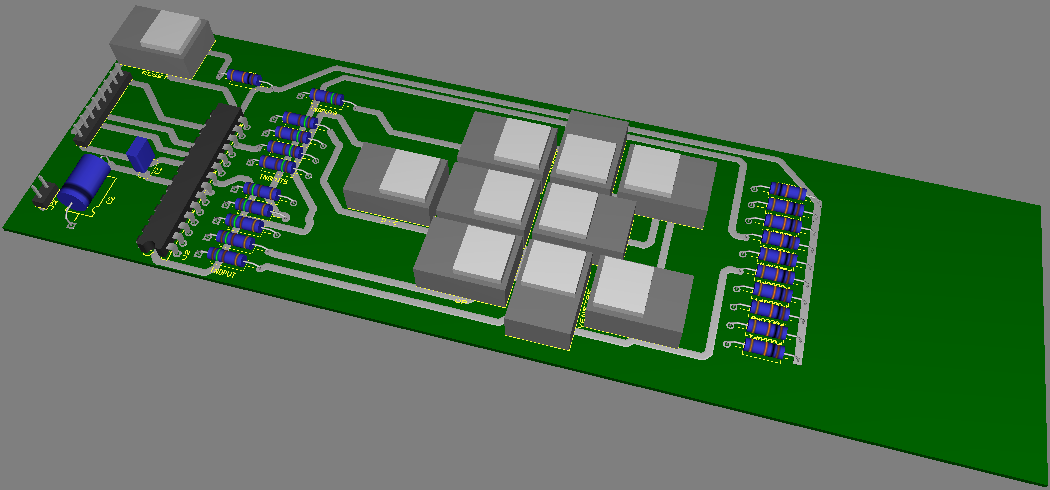
\includegraphics[scale=0.5]{Print3D}
\caption{Det færdige print}
\label{fig: Print3D}
\end{figure}
Det endelige layout kan ses på Figur \ref{fig: Print3D}.
Layouted er forsøgt holdt simpelt. knapperne til brugeren er placeret så de minder om pilene på et tastatur, dog med op/ned funktioner og autoland.
Printet er aflangt så det er til at holde som en fjernbetjening og derved kan styres med en hånd.
Radioen er placeret forrest på fjernbetjeningen, for at brugeren dæmper/skærmer mindst muligt for signalet.  


\end{document}
